\chapter{Introduction}

\begin{comment}
This chapter puts the work into context. Having read it, the reader should be left in no doubt as to:

- the topic area to which the work applies
- why the work is being done
- what else has been done in the area and by whom
 - how the author proposes to tackle the problem: The project proposal is often expressed in terms of a main objective and possibly one or more additional objectives. It is useful to define "milestones" or "sub-goals" that mark the progress towards the objectives. 
 - It is common to end this chapter with a brief overview of each of the subsequent chapters of the report.
\end{comment}

Traditionally the management of personal finances is performed by viewing bank statements provided by the users bank, however, even in this modern age of 'internet banking' banks offer a limited set of tooks that mimic the paper statements that would have been sent in the past.

This project sets out to build an online application that can be used to manage personal finances. There are two main parts of the project; firstly Users can upload  bank statements, which are displayed and navigated in an intuitive manner; secondly, once the application has enough historical data, predicting the users future outflow.

\section{Motivation}
% \plan{Help make managing finances easier, basic survey of people + appendix with details, any relevant paperts}
There are four main steps when producing and using a budget, recording previous expenses, sorting these into categories
using this historical information to guess future expenditure and evaluate accuracy of these predictions and using new information to update them.

Since the liquidity crisis of 2009 \cite{gore2010}, budgets have been squeezed and the average persons personal disposable income has fallen, hitting a nine-year low in 2012\cite{barnard2012households}. With experts suggesting that ``Budgets are essential for financial planning''\cite{wsj2013budget}, research suggesting that personal budgets lead to a ``positive impact on ``mental wellbeing''\cite{tlap2013budget} and guides from UCAS, the UoM SU Advice Centre and The Manchester University Crucial Guide encouraging use of budgeting, it is clear that producing a budget is of benefit.

However, in an informal survey\footnote{Appendix \ref{app:budgetsurvey}} the majority of students surveyed, did not make a budget. An easier way to produce a budget can hopefully increase the amount of students relying on one.

Increasing use of debit cards\cite{bbc2010debit} means that bank statements contain more and more information about where people spend their money. With access to those bank statements now provided online, with most UK banks offering the option to export \gls{transaction} history, individual users can collate a database of their personal spending habits.

The increasing availability of this data, combined with more detailed transaction history makes it possible to automate the four main steps of producing a budget, and this is the idea behind the project.

\section{Existing work in this area}

\subsection{Management}
There are several other applications implement management features found in this project, most notably Lloyds TSB Money Manager \cite{lloyds2014money}, which was the first money management application provided by a UK bank.

The service is available to Lloyds TSB current account holders as part of their online banking and offers several key features, however all of the features revolve around documenting historical spending.

\begin{itemize}
\item Categorising spending
\item Creating spending plans per category.
%\item View dates money came in and out in a calendar
\item Viewing money spent per category
\item Track progress of budget targets
\end{itemize}

\begin{figure}[h]
    \centering
    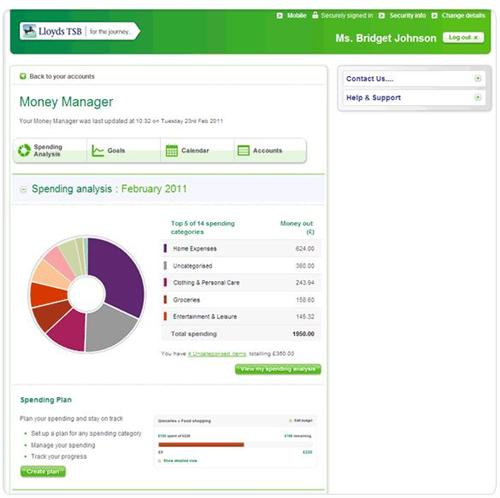
\includegraphics{moneymanagerchart}
    \caption{Spending Analysis on Money Manager \parencite{lloyds2014money}}
    \label{fig:moneymanager}
\end{figure}

Mint.com is a US only personal finance service that provides features similar to those provided by LLoyds. They include the ability to login to your bank account to have your statements pulled over automatically.

There are also many mobile apps that provide this management facility, however all those investigated when planning the project had the same drawback, the user had to manually enter all of their transactions and set categories for them \cite{spendee2014spendee,budgt2013budgt,bluetags2014pocket}.

\subsection{Prediction}

\todo[inline]{Make this make sense}
Predicting future expenditure given previous history is notoriously hard. There have been several different approaches to this in the past in the context of personal finance, but by opening up to other finance predictions such as those on the stock market, there is a lot more research.
\todo[inline]{Finish this}

\section{Aims and Objectives}
\plan{Things I set out to do, designed by talking to people to get an idea of features they would like}

The key objectives of this project can be split into three parts, the management of statements, making prediction using those statements and ensuring a high level of security.

\subsection{Statements Management}
Implement an intuitive way to view and manage personal finances.
There are several key parts to this, upload and parsing of transactions from statements downloaded from a bank, resolving the references found on the statement to the transactor they represent and categorising the transactions.
    
\subsection{Predictions}
Make predictions of future transactions that a user will make using a model that is fitted to their spending behaviour, the application will need to predict whether or not spending will occur and how much money will be spent.
Using

\subsection{Security}
As the application will deal with information of a sensitive nature strong security techniques are particularly important.
The project should take this into account, considering possible attack vectors and taking steps to mitigate those attacks.

\section{Overview of Report}
\plan{This report covers some of the key design decisions, implementation decisions and then what the application does}
